\section{UML проектирование}

\begin{figure}[h]
\center{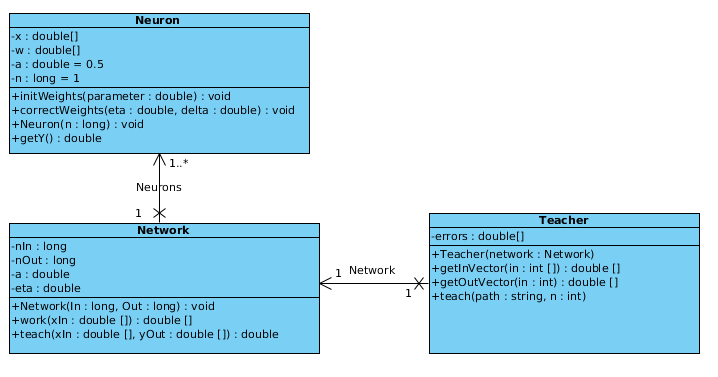
\includegraphics[width=1\linewidth]{uml}}
\caption{Диаграмма классов программного решения.}
\label{ris:UML}
\end{figure}

Первоначальной стадией разработки программного продукта является стадия проектирования.
В качестве проектного CASE-средства был выдран продукт Visual Paradigm.
С помощью его было составлена диаграмма классов (см. рис. ~\ref{ris:UML}), на основе которой был сгенерирован начальный код программного решения.